\documentclass[pdf]{beamer}
\mode<presentation>{}
\usepackage{minted}
\usepackage{tikz}
\usepackage{pgffor} %% gives looping with \foreach
\usepackage[absolute,overlay]{textpos}
\usepackage{lmodern} %% scalable latin characters
\usetikzlibrary{arrows,shapes,backgrounds}
\usepackage{multirow}

%% it seems that beamer and descriptions can be a bit
%% tricky, so we need to define some things ourselves
\defbeamertemplate{description item}{align left}{\insertdescriptionitem\hfill}

%% I detest indentation in footnotes etc, so try this:
\makeatletter
\renewcommand\@makefntext[1]{\noindent\makebox[0em][r]{\@makefnmark}\tiny#1}
\makeatother
%% the makeatletter and makeatother are required to allow me to
%% to change the macro beginning with an @. (though when I call it
%% I don't use the @ ... 

%% a command to define a subheading
\newcommand\subHeading[1]{
  \par\bigskip {\Large\bfseries#1}\par\smallskip
}

%% define styles for different codes
\definecolor{mintedBg}{rgb}{0.95, 0.95, 0.95}
\definecolor{blockBg}{rgb}{0.6, 0.6, 0.95}
\newminted{cpp}{linenos, bgcolor=blockBg, fontsize=\footnotesize}
%% then use \begin{cppcode}
\newminted{c}{linenos, bgcolor=mintedBg, fontsize=\footnotesize}
\newminted{perl}{linenos, bgcolor=mintedBg, fontsize=\footnotesize}
\newminted{r}{linenos, bgcolor=mintedBg, fontsize=\footnotesize}


\title{Questions for students}
\subtitle{Introduction to B1229F 2015 (2)}
\author{Martin Jakt}

\setlength\parskip{0.5em}
\begin{document}

\begin{frame}
  \titlepage
\end{frame}

\begin{frame}{Questions for you}
  A set of questions for me to determine:
  \begin{itemize}
    \item What I need to introduce in the course.
    \item From what level I can start the course.
    \item What I should stay away from.
  \end{itemize}
  Some of these may seem a bit silly...
\end{frame}

\begin{frame}{DNA}
  What is DNA?

  What is the difference between DNA \& RNA?
\end{frame}

\begin{frame}{Protein}
  What is a protein molecule?

  What interesting properties do proteins have?
\end{frame}

\begin{frame}{Molecular biology terms}
  \begin{itemize}
    \item Gene
    \item Allele
    \item Transcription
    \item Translation
    \item cis acting element
    \item trans acting factor
    \item transcription factor
    \item ribosome
    \item codon
    \item mRNA
    \item tRNA
    \item Protein kinase
  \end{itemize}
\end{frame}

\begin{frame}{more terms}
  \begin{itemize}
    \item PCR (polymerase chain reaction)
    \item oligonucleotide
    \item hybridisation
    \item antibody
    \item enzyme
    \item fluorescent
    \item DNA / RNA polymerase
    \item in situ hybridisation
    \item Number (!?)\footnote{the set of all equivalent sets}
    \item Information
  \end{itemize}
\end{frame}

\begin{frame}[fragile]{Chemical structures}
  What is this?
  \begin{figure}[ht]
  \begin{tikzpicture}[scale=0.5]
    \draw [help lines,opacity=0] (0,0) grid(24,10);
%    \foreach \x in {1, 2,...,19}
%      \node [font=\small]  at (\x,1) {\x};
%      \draw [->] (\x,0) -- (\x,1);
%    \foreach \y in {2,3,...,9}
%      \node [font=\small] at (19,\y) {\y};
%    \node [inner sep=0pt,above right]
    \node [above right] at (3,3)
          {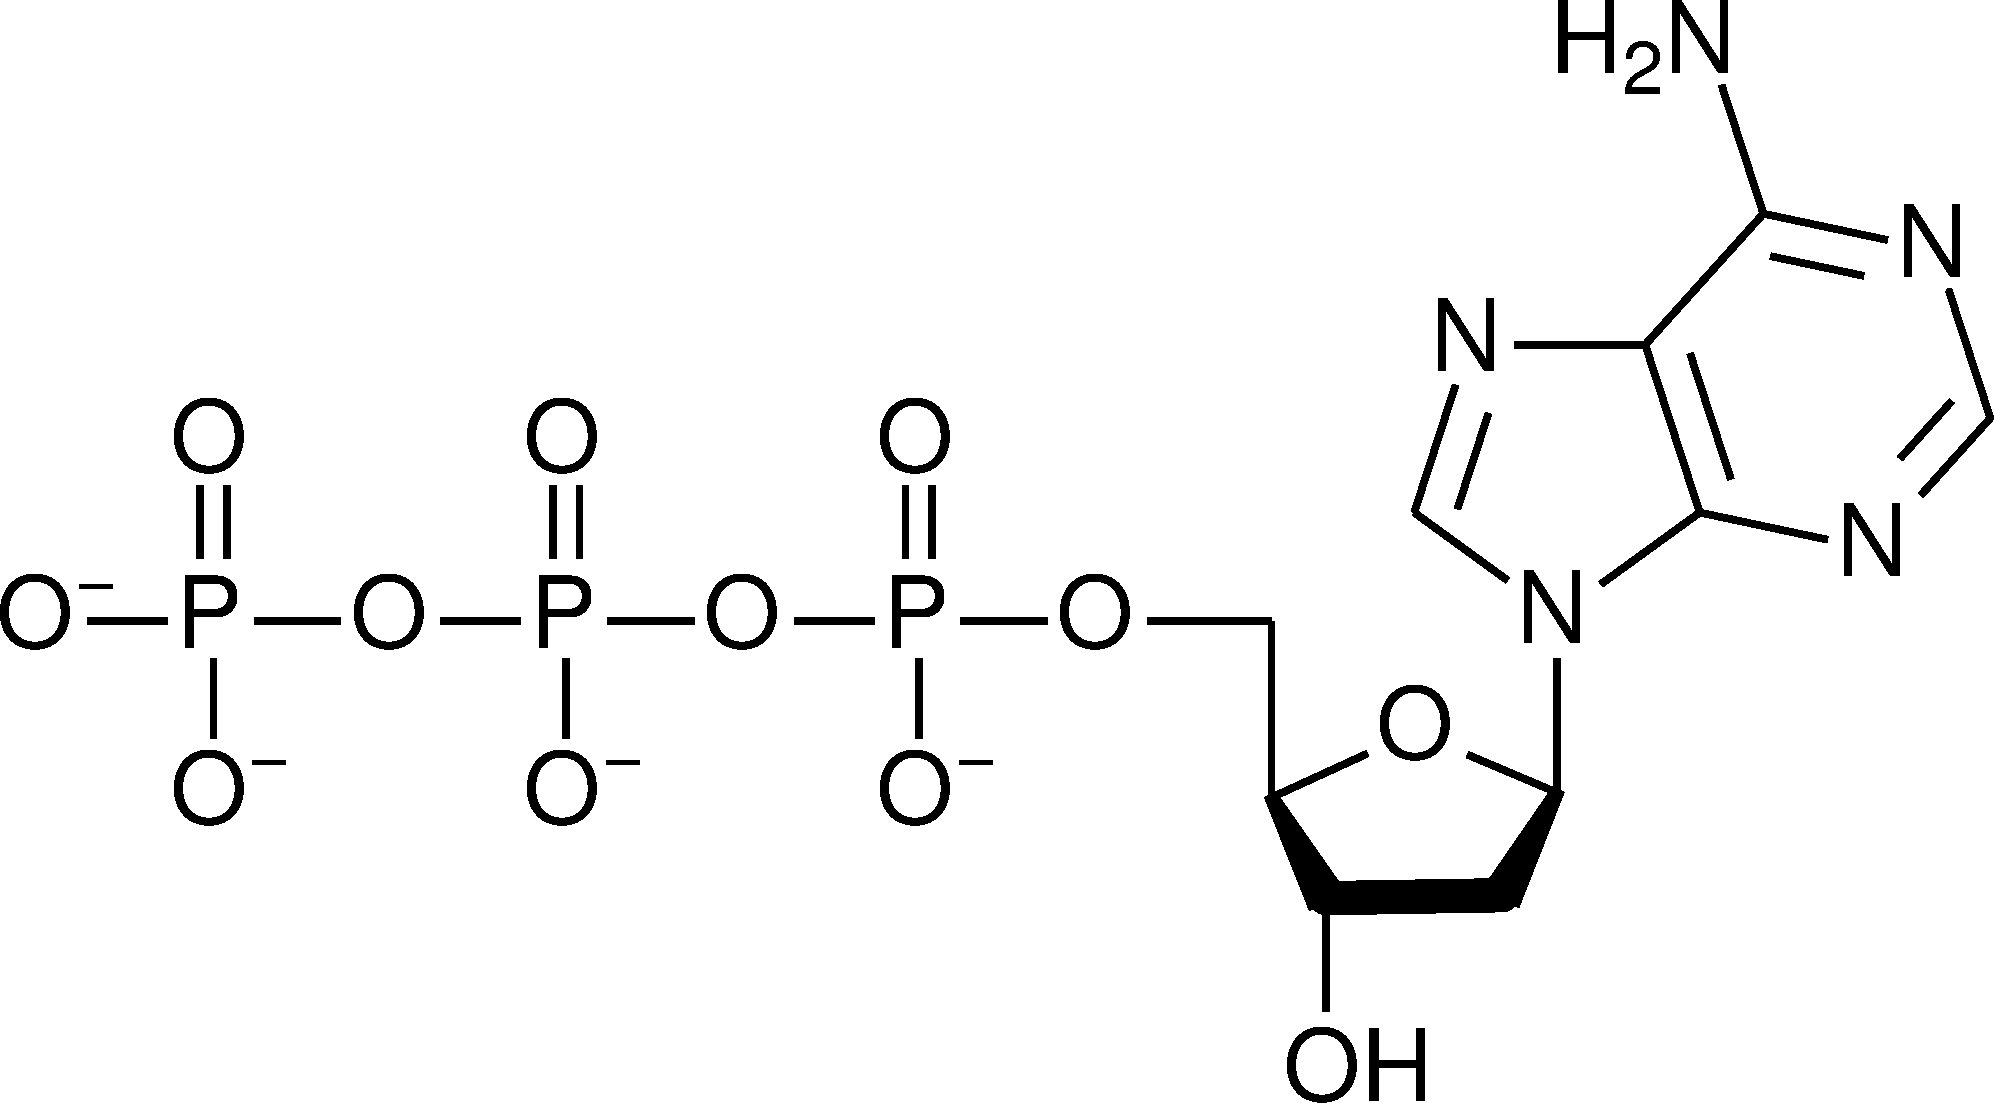
\includegraphics[width=0.5\textwidth]{images/dATP_structure.pdf}};
    \draw <2> [<-,blue] (11.5, 4.2) -- (15.5,3) node [right, align=left] {carbon\\atoms};
    \draw <2> [->,blue] (15.5,3) to [out=180, in=270] (12.5,6.3);
    \draw <2> [->,blue] (15.5,3) to [out=90, in=0] (14.1, 7);
    \draw <3> [->,blue] (15.5,3) node [right, align=left] {nitrogen\\atoms} 
                    to [out=90,in=0] (14.1, 8);
    \draw <3> [->,blue] (15.5,3) to [out=195,in=320] (13.4, 6);
    \draw <3> [->,blue] (15.5,3) to [out=180,in=315] (12,5.8);
    \draw <4> [->,blue] (15.5,3) node [right, align=left, font=\small] {carbon-carbon\\double bonds}
                    to [out=180,in=210] (12.2, 6.8);
    \draw <4> [->,blue] (15.5,8.5) node [right, align=left, font=\small] {carbon-nitrogen\\double bonds}
                    to [out=180,in=85] (13.2,8.2);
    \draw <4> [->,blue] (15.5,8.5) to [out=270,in=315] (14,6.5);
    \draw <5> [->,blue] (15.5,3.5) node [right, align=left, font=\small] {implicit\\hydrogen\\atoms}
                    to [out=180,in=270] (11.55,4.2);
    \draw <5> [->,blue] (15.5,3.5) to [out=170,in=0] (11.9,5);
    \draw <5> [->,blue] (15.5,3.5) to [out=100,in=0] (14.1,7.0);
    \draw <5> [->,blue] (15.5,3.5) to [out=90,in=0] (14,8.5) to [out=180,in=135] (10.9,6.5);
  \end{tikzpicture}
  \end{figure}
\end{frame}

\begin{frame}{Basic equations}
  
  $$
  \mu = \frac{1}{N} \sum_{i=1}^{N} x_i
  $$
  
  $$
  \sigma=\sqrt{\frac{1}{N} \sum_{i=1}^N(\bar{x}-x_i)^2}
  $$

  $$
  z = \frac{x - \mu}{\sigma}
  $$
\end{frame}

\begin{frame}{Distributions}
  \begin{columns}
    \begin{column}{0.5\textwidth}
      \begin{figure}[ht]
      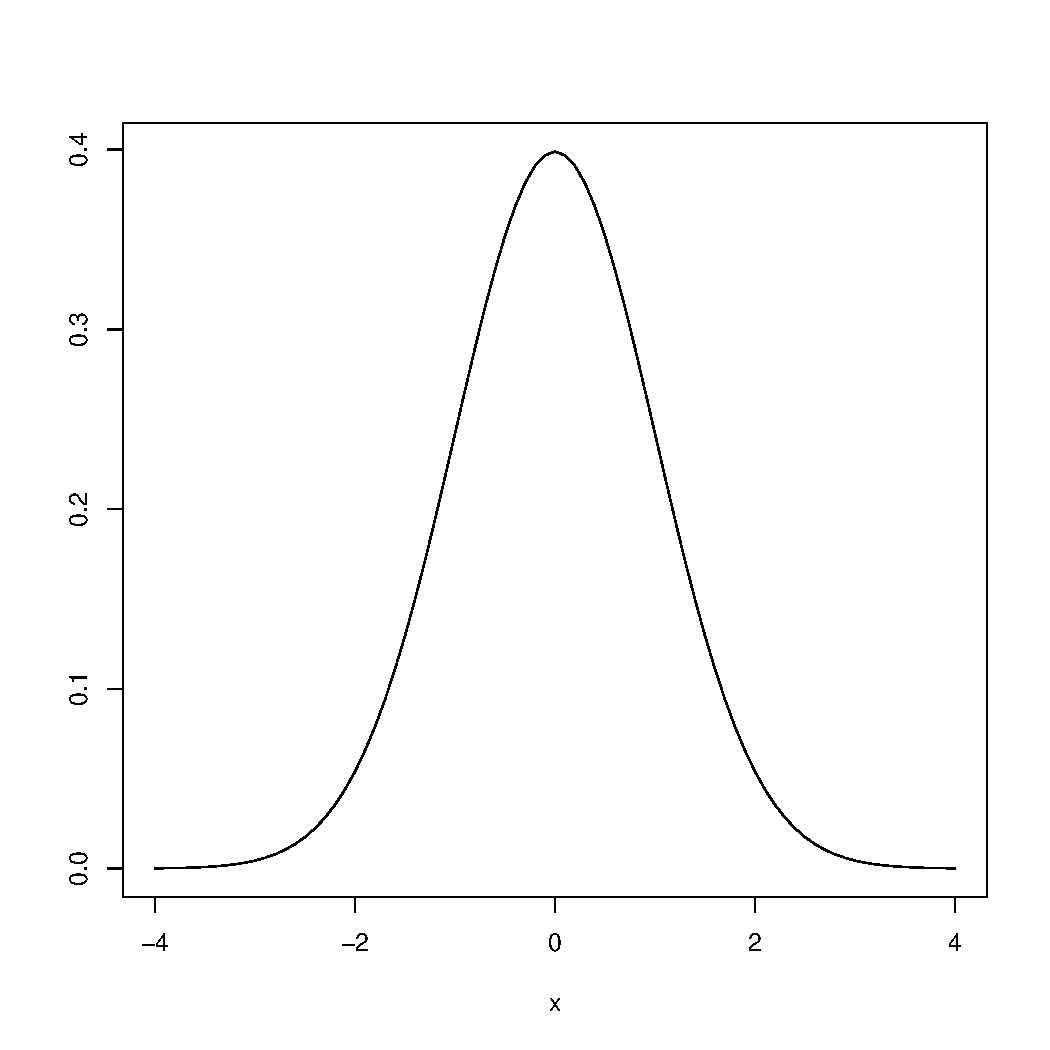
\includegraphics[width=\textwidth]{images/normal.pdf}
      \end{figure}
      \visible<2>{Normal distribution}
    \end{column}
    \begin{column}{0.5\textwidth}
      \begin{figure}[ht]
      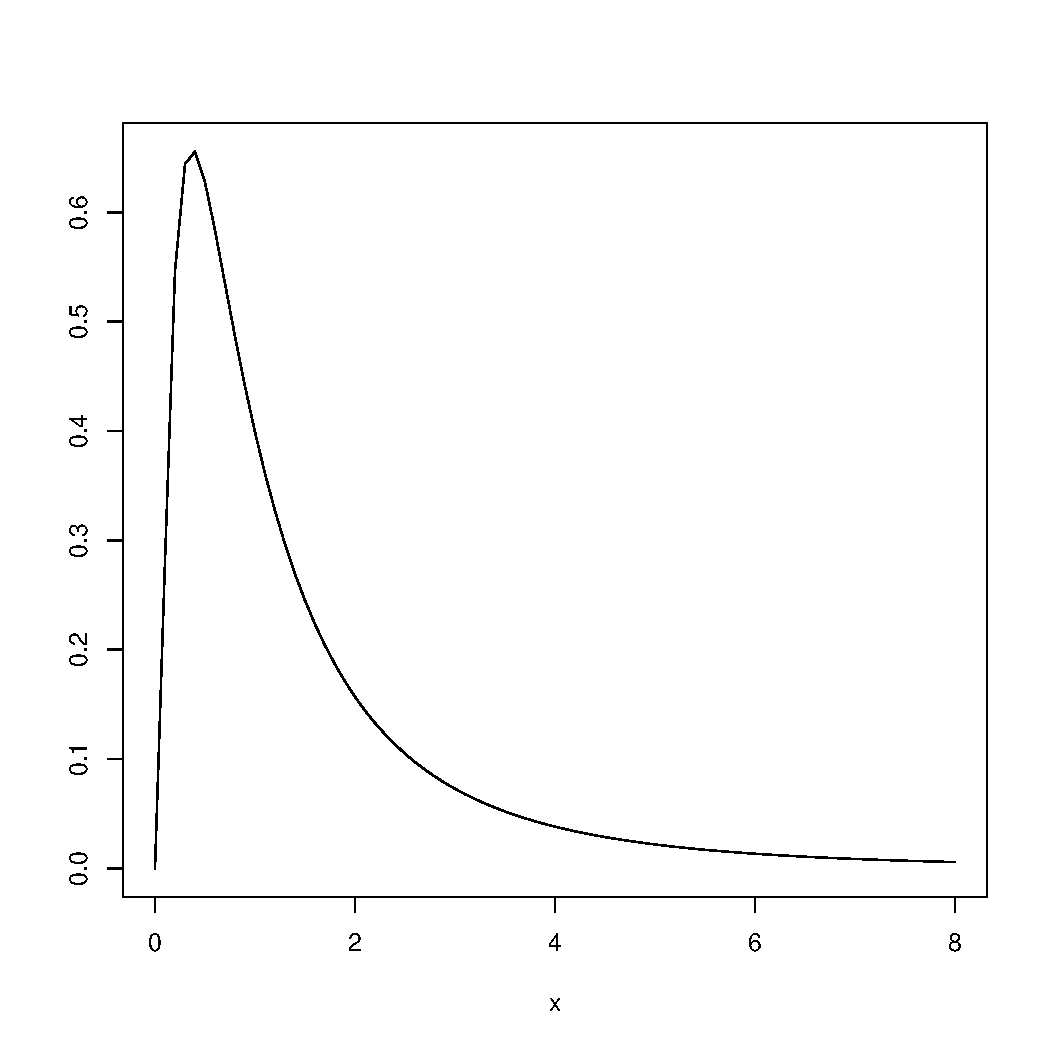
\includegraphics[width=\textwidth]{images/log_normal.pdf}
      \end{figure}
      \visible<2>{Log normal distribution}
    \end{column}
  \end{columns}
\end{frame}

\begin{frame}[fragile]{Reading code}
  \subHeading{Perl}
  \begin{perlcode}
    #!/usr/bin/perl -w
    for($i=0; $i < 10; $i++){
      print $i, "\t", $i * $i, "\n";
    }
  \end{perlcode}
  \subHeading{R}
  \begin{rcode}
    for(i in 1:10){
      cat(paste(i, i^2, sep='\t'), '\n')
    }
  \end{rcode}
\end{frame}

\end{document}
